% Revised academic cover and source layout for Oday AL Fakhoury.
% The technical report body is retained from the BaladiNet deployment report.

\documentclass[11pt,a4paper,oneside]{report}

% ============================================================
% BaladiNet Technical Implementation and Deployment Report
% Compiled with XeLaTeX
% ============================================================

\usepackage{fontspec}
\usepackage{graphicx}
\IfFontExistsTF{Liberation Serif}{\setmainfont{Liberation Serif}}{\setmainfont{TeX Gyre Termes}}
\IfFontExistsTF{Liberation Mono}{\setmonofont{Liberation Mono}}{\setmonofont{DejaVu Sans Mono}}

\usepackage[a4paper,top=2.45cm,bottom=2.4cm,left=2.55cm,right=2.55cm,headheight=15pt]{geometry}
\usepackage{setspace}
\setstretch{1.18}
\usepackage{microtype}
\usepackage{titlesec}
\usepackage{fancyhdr}
\usepackage{enumitem}
\usepackage{array,tabularx,booktabs,longtable,multirow}
\usepackage{float}
\usepackage{listings}
\usepackage{xcolor}
\usepackage{caption}
\usepackage{url}
\usepackage{xurl}
\usepackage{hyperref}
\usepackage{bookmark}
\usepackage{tikz}
\usetikzlibrary{arrows.meta,positioning,shapes.geometric}

\definecolor{Navy}{HTML}{17365D}
\definecolor{Teal}{HTML}{0F766E}
\definecolor{PaleBlue}{HTML}{EAF1F8}
\definecolor{PaleGray}{HTML}{F3F4F6}
\definecolor{DarkGray}{HTML}{374151}
\definecolor{Green}{HTML}{166534}
\definecolor{Amber}{HTML}{92400E}

\hypersetup{
  colorlinks=true,
  linkcolor=Navy,
  urlcolor=Teal,
  citecolor=Navy,
  pdftitle={BaladiNet: Design and Deployment of a Municipal Network Infrastructure Management Platform},
  pdfauthor={Oday AL Fakhoury},
  pdfsubject={Network Administration (10686213) - Technical Implementation and Deployment Report},
  pdfkeywords={BaladiNet, NetBox, municipal networks, IPAM, DCIM, PostgreSQL, Redis}
}
\urlstyle{same}

\titleformat{\chapter}[display]
  {\normalfont\bfseries\color{Navy}\Huge}
  {\chaptertitlename\ \thechapter}{10pt}{\Huge}
\titleformat{\section}
  {\normalfont\Large\bfseries\color{Navy}}{\thesection}{0.65em}{}
\titleformat{\subsection}
  {\normalfont\large\bfseries\color{Teal}}{\thesubsection}{0.65em}{}

\pagestyle{fancy}
\fancyhf{}
\fancyhead[R]{\small BaladiNet}
\fancyhead[L]{\small Technical Implementation Report}
\fancyfoot[L]{\small Network Administration (10686213) -- BaladiNet}
\fancyfoot[R]{\small Page \thepage}
\renewcommand{\headrulewidth}{0.4pt}
\renewcommand{\footrulewidth}{0pt}

\setlist[itemize]{itemsep=3pt,topsep=4pt,leftmargin=1.5em}
\setlist[enumerate]{itemsep=3pt,topsep=4pt,leftmargin=1.7em}

\newcolumntype{Y}{>{\raggedright\arraybackslash}X}
\newcolumntype{L}[1]{>{\raggedright\arraybackslash}p{#1}}

\lstdefinestyle{terminal}{
  basicstyle=\ttfamily\small,
  breaklines=true,
  columns=fullflexible,
  keepspaces=true,
  showstringspaces=false,
  frame=single,
  rulecolor=\color{DarkGray},
  backgroundcolor=\color{PaleGray},
  xleftmargin=4pt,
  xrightmargin=4pt,
  aboveskip=8pt,
  belowskip=8pt
}
\lstset{style=terminal}

\newcommand{\code}[1]{\texttt{\detokenize{#1}}}
\newcommand{\pathcode}[1]{\path{#1}}
\newcommand{\Completed}{\textcolor{Green}{\textbf{Completed and verified}}}
\newcommand{\Pending}{\textcolor{Amber}{\textbf{Pending}}}
\newcommand{\NotImplemented}{\textcolor{DarkGray}{\textbf{Not implemented}}}
\newcommand{\ReportDate}{26 November 2026}

\begin{document}

% ============================================================
% COVER
% ============================================================
\begin{titlepage}
\thispagestyle{empty}
\begin{center}
\vspace*{0.15cm}

% University identity
\includegraphics[width=4.15cm]{university_logo.png}\\[0.30cm]
{\Large\bfseries An-Najah National University}\\[0.12cm]
{\large\bfseries Faculty of Information Technology and Artificial Intelligence}\\[0.16cm]
{\large Network Administration (10686213)}\\[0.10cm]
{\large First Semester 2026--2027}\\[0.45cm]

\rule{0.88\textwidth}{1.0pt}\\[0.48cm]

% Proposed project title
{\Huge\bfseries\color{Navy} BALADINET}\\[0.20cm]
{\LARGE\bfseries Design and Deployment of a Municipal Network Infrastructure Management Platform}\\[0.28cm]
{\large\bfseries Technical Implementation and Deployment Report}\\[0.65cm]

% Student and course information
\renewcommand{\arraystretch}{1.28}
\begin{tabular}{@{}>{\bfseries}r l@{}}
Student Name: & Oday AL Fakhoury\\
Registration Number: & 12400455\\
Instructor: & Jehad Hamamreh\\
Course: & Network Administration (10686213)\\
Semester: & First Semester 2026--2027\\
\end{tabular}

\vspace{0.60cm}
\begin{tabular}{@{}>{\bfseries}r l@{}}
Base software: & NetBox Community 4.7.5\\
Operating environment: & Ubuntu 24.04.4 LTS on VMware Workstation\\
Deployment type: & Local virtual-machine laboratory deployment\\
Report date: & \ReportDate\\
\end{tabular}

\vfill

\begin{minipage}{0.88\textwidth}
\centering
\normalsize
This report documents the implementation and verification of the NetBox platform selected as the technical foundation for BaladiNet. It records the deployment work completed in the laboratory environment and identifies the remaining activities required to populate, customize, and validate the municipal network management solution.
\end{minipage}

\vspace{0.55cm}
{\color{Teal}\rule{0.48\textwidth}{0.8pt}}\\[0.18cm]
{\small Academic Project Report -- Network Administration}
\end{center}
\end{titlepage}

\pagenumbering{roman}

% ============================================================
% ABSTRACT
% ============================================================
\chapter*{Abstract}
\addcontentsline{toc}{chapter}{Abstract}

BaladiNet is an academic project that applies the open-source NetBox platform to the proposed management and documentation of municipal network infrastructure for the target municipality, Palestine. The intended system provides a centralized source of truth for sites, network devices, interfaces, IP address allocations, VLANs, racks, cables, and telecommunications circuits. The project addresses a common infrastructure-management challenge: technical records can become distributed across spreadsheets, local documents, and individual staff knowledge, making inventory, troubleshooting, and maintenance more difficult.

The implementation work documented in this report established a working NetBox 4.7.5 deployment inside an Ubuntu 24.04.4 LTS virtual machine hosted by VMware Workstation. The environment was prepared with Python 3.12.3, PostgreSQL 16.15, Redis 7.0.15, the required system development libraries, Gunicorn, systemd service units, Nginx, and a locally generated self-signed TLS certificate. A dedicated PostgreSQL database and role were created for NetBox, the application configuration was prepared, database migrations completed through the official upgrade script, and a NetBox administrator account was created.

The deployment was verified through service-state checks, a successful PostgreSQL authentication test, a successful Gunicorn response on the local application port, successful Nginx configuration validation, and HTTP 200 responses through the HTTPS endpoint. The administrator then opened the NetBox interface from the Windows host and successfully signed in.

This report distinguishes platform deployment from completion of the full municipal solution. At the reporting date, no official municipal inventory had been imported, and no municipal sites, devices, VLANs, prefixes, IP addresses, cables, or circuits had yet been entered. The Python REST API automation and Cisco Packet Tracer simulation also remain future implementation tasks. Therefore, the verified result is a functioning NetBox platform ready for controlled data population and customization, rather than a completed production deployment for the municipality.

\noindent\textbf{Keywords:} BaladiNet, NetBox, municipal network management, DCIM, IPAM, PostgreSQL, Redis, Python, Ubuntu, network documentation.

\clearpage
\tableofcontents
\listoftables
\clearpage
\pagenumbering{arabic}

% ============================================================
\chapter{Project Overview}

\section{Background}
Municipal organizations depend on interconnected information and communication technology infrastructure. Typical components include routers, switches, servers, wireless access points, network interfaces, IP subnets, VLANs, racks, patch panels, cables, and external connectivity circuits. As an organization grows or its infrastructure changes, the information describing these components may be stored in separate spreadsheets, documents, diagrams, or staff-maintained records.

BaladiNet proposes the use of NetBox as a centralized platform for documenting this infrastructure. NetBox provides data models for data-center infrastructure management (DCIM), IP address management (IPAM), device inventory, cabling, circuits, and programmable interfaces. Its capabilities make it suitable as the base platform for a municipal network documentation system.

\section{Problem Statement}
The project is based on the proposed problem of fragmented or incomplete network infrastructure records in a municipal environment. If device locations, IP assignments, VLAN definitions, interface connections, and circuit information are maintained in separate records, technical staff may face additional effort when identifying assets, tracing connections, planning changes, or preparing maintenance activities.

This is the problem scenario that BaladiNet is designed to address. The work documented here does not claim that the target municipality has confirmed these specific deficiencies. Confirmation of the municipality's actual operational situation requires consultation with authorized municipal IT personnel and review of approved records.

\section{Proposed Solution}
BaladiNet uses the upstream NetBox Community application as its core platform. The planned municipal deployment will organize infrastructure information into related records rather than independent lists. For example, a device can be associated with a site, a device role, a manufacturer and model, interfaces, IP addresses, VLAN assignments, racks, and cable terminations.

The initial implementation intentionally uses standard NetBox functionality. No custom Django application or NetBox plugin has been developed as part of the work completed to date.

\section{Project Objectives}
The objectives are:
\begin{enumerate}
  \item Prepare an isolated Linux environment for the project without installing its application stack directly on Windows.
  \item Install a stable, identified NetBox release and its required dependencies.
  \item Configure PostgreSQL and Redis for application data and background processing.
  \item Deploy NetBox behind Gunicorn and Nginx.
  \item Verify that the application can be reached from the Windows host.
  \item Establish a foundation for municipal site, device, IPAM, VLAN, and cabling records.
  \item Define the next steps for authorized data collection, Python API automation, network simulation, and final project validation.
\end{enumerate}

\section{Scope of This Report}
This report covers the work actually performed and verified during the platform deployment. It includes the virtual machine preparation, source archive transfer, dependency installation, database configuration, NetBox installation, service deployment, HTTPS configuration, troubleshooting, and acceptance tests. It also documents the remaining implementation work.

% ============================================================
\chapter{Implementation Scope and Status}

\section{Completed Deployment Scope}
The following items were completed:
\begin{itemize}
  \item Ubuntu virtual machine preparation and an initial VMware snapshot.
  \item Verification of CPU, memory, storage, operating-system version, and network configuration.
  \item Installation and verification of Python, PostgreSQL, Redis, curl, and NetBox system dependencies.
  \item Acquisition of the official NetBox 4.7.5 source archive and transfer to Ubuntu using a read-only VMware shared folder.
  \item Creation of the project working directory and a separate versioned installation directory.
  \item PostgreSQL database and role creation, ownership assignment, schema privilege verification, and successful login testing.
  \item NetBox configuration file creation, local secret generation, and database/Redis configuration.
  \item NetBox upgrade script execution and superuser creation.
  \item Gunicorn, systemd, Nginx, and local HTTPS configuration.
  \item Successful browser access and administrator login from Windows.
\end{itemize}

\section{Items Not Completed at the Reporting Date}
The following tasks remain outside the verified deployment milestone:
\begin{itemize}
  \item Importing official or approved municipal site and building information.
  \item Creating municipal device records, device types, manufacturers, roles, racks, and interfaces.
  \item Entering the municipality's real VLANs, prefixes, IP addresses, VRFs, and circuit records.
  \item Documenting real cable paths and device-to-device connections.
  \item Creating BaladiNet-specific custom fields, tags, permissions, and operational workflows.
  \item Developing a Python program that uses the NetBox REST API.
  \item Creating and testing the municipal network model in Cisco Packet Tracer.
  \item Establishing and testing a repeatable backup and restore procedure.
  \item Replacing the self-signed laboratory certificate with a trusted certificate if the system is exposed beyond the local laboratory.
  \item Performing a full security review and production-readiness assessment.
\end{itemize}

\section{Data Integrity and Evidence Policy}
No municipal data was invented or represented as real. All future demonstration records must be clearly marked as synthetic or demonstration data unless they are obtained from an authorized municipal source. Network scanning, device configuration collection, or access to operational network equipment must only be performed with explicit authorization.

% ============================================================
\chapter{System Architecture and Environment}

\section{Virtualization and Operating System}
The platform was deployed inside VMware Workstation using Ubuntu 24.04.4 LTS. This approach kept the project application stack inside a virtual machine rather than installing PostgreSQL, Redis, NetBox, or Nginx directly on Windows.

A VMware snapshot named \pathcode{BaladiNet-Before-Installation} was created before installation work began. This snapshot preserved the initial Ubuntu state. A later post-deployment snapshot was not documented as completed.

\section{Virtual Machine Resources}
The initial resource checks produced the following results.

\begin{table}[H]
\centering
\caption{Initial virtual-machine resource profile}
\begin{tabularx}{\textwidth}{L{0.42\textwidth}Y}
\toprule
\textbf{Resource} & \textbf{Observed value}\\
\midrule
Operating system & Ubuntu 24.04.4 LTS\\
Virtual CPU & 2 logical CPUs\\
Memory & Approximately 7.7 GB RAM\\
Swap & 4 GB\\
Virtual disk capacity & 40 GB\\
Available disk space at initial check & Approximately 26 GB\\
Network interface & \pathcode{ens33}\\
VM IPv4 address during deployment & \pathcode{192.168.227.131}\\
VMware NAT gateway & \pathcode{192.168.227.2}\\
\bottomrule
\end{tabularx}
\end{table}

These resources were sufficient for the small academic laboratory deployment. They should not be interpreted as a capacity plan for a production municipal service. Production sizing would require information about the number of devices, users, API operations, background jobs, data retention, and expected growth.

\section{Software Stack}
\begin{table}[H]
\centering
\caption{Installed and verified software components}
\begin{tabularx}{\textwidth}{L{0.30\textwidth}L{0.24\textwidth}Y}
\toprule
\textbf{Component} & \textbf{Version} & \textbf{Role}\\
\midrule
Ubuntu & 24.04.4 LTS & Guest operating system\\
Python & 3.12.3 & NetBox application runtime\\
PostgreSQL & 16.15 & Relational database\\
Redis & 7.0.15 & Background task queue and caching support\\
curl & Installed; exact version not recorded & HTTP/HTTPS diagnostics\\
NetBox & 4.7.5 & Core infrastructure documentation platform\\
Gunicorn & Installed in NetBox virtual environment & WSGI application server\\
Nginx & Installed; exact package version not recorded & HTTPS reverse proxy and static-file server\\
OpenSSL & Installed; exact package version not recorded & Local self-signed TLS certificate generation\\
\bottomrule
\end{tabularx}
\end{table}

NetBox 4.7 supports Python 3.12--3.14, PostgreSQL 15 or later, and Redis 6.0 or later. The versions verified in this deployment meet those stated minimum requirements \cite{netbox-install,upgrade}.

\section{Network Mode}
VMware NAT was used for the final deployment. A temporary Bridged-mode test did not provide the guest with an IPv4 address or a default route. The adapter was therefore returned to NAT. The guest subsequently used the address \pathcode{192.168.227.131} during the final local access tests.

The address is a laboratory NAT address and may change if the VMware network or guest lease changes. It is not a permanent municipal service address.

\section{Application Architecture}
The deployed request path is:

\begin{figure}[H]
\centering
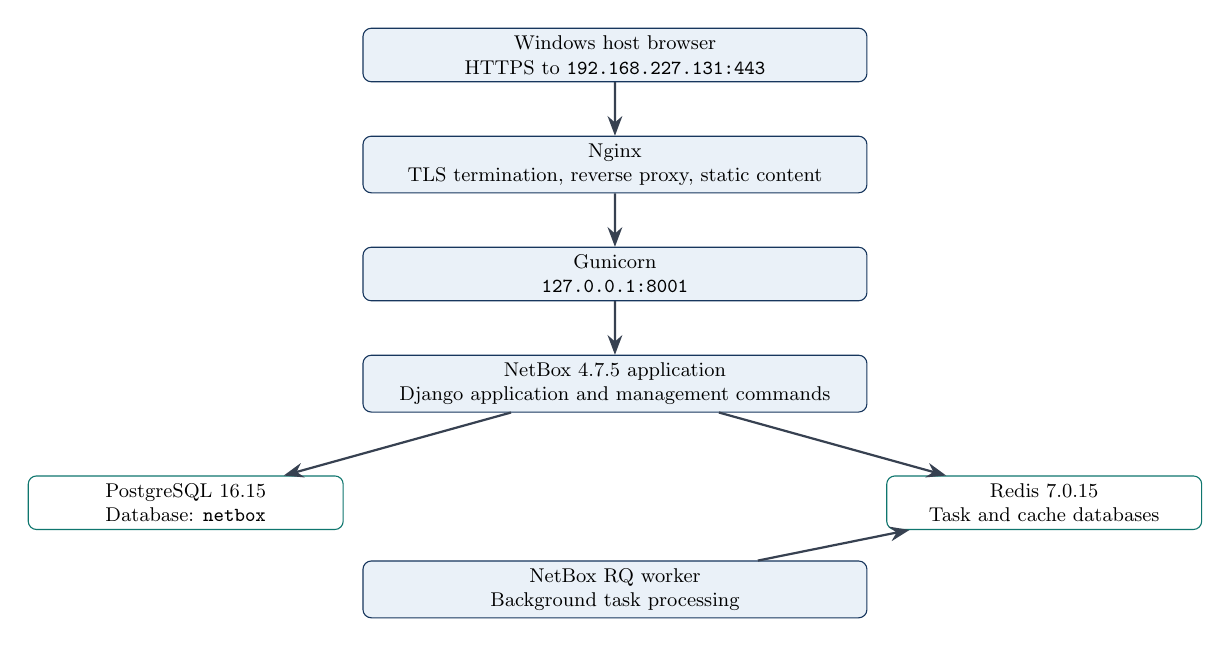
\begin{tikzpicture}[scale=0.80,transform shape,
  node distance=0.85cm,
  box/.style={draw=Navy, fill=PaleBlue, rounded corners=3pt, align=center, minimum width=8.0cm, minimum height=0.85cm, font=\small},
  db/.style={draw=Teal, fill=white, rounded corners=3pt, align=center, minimum width=5.0cm, minimum height=0.85cm, font=\small},
  arr/.style={-{Stealth[length=2.5mm]}, thick, color=DarkGray}
]
\node[box] (client) {Windows host browser\\HTTPS to \texttt{192.168.227.131:443}};
\node[box, below=of client] (nginx) {Nginx\\TLS termination, reverse proxy, static content};
\node[box, below=of nginx] (gunicorn) {Gunicorn\\\texttt{127.0.0.1:8001}};
\node[box, below=of gunicorn] (app) {NetBox 4.7.5 application\\Django application and management commands};
\node[db, below left=1.0cm and 0.3cm of app] (postgres) {PostgreSQL 16.15\\Database: \texttt{netbox}};
\node[db, below right=1.0cm and 0.3cm of app] (redis) {Redis 7.0.15\\Task and cache databases};
\node[box, below=1.25cm of app, yshift=-1.1cm] (rq) {NetBox RQ worker\\Background task processing};
\draw[arr] (client) -- (nginx);
\draw[arr] (nginx) -- (gunicorn);
\draw[arr] (gunicorn) -- (app);
\draw[arr] (app) -- (postgres);
\draw[arr] (app) -- (redis);
\draw[arr] (rq) -- (redis);
\end{tikzpicture}
\caption{Logical architecture of the local BaladiNet deployment}
\end{figure}

Nginx receives the browser request over HTTPS and forwards application requests to Gunicorn. Gunicorn serves the NetBox application on the loopback interface. NetBox stores structured data in PostgreSQL and uses Redis for background task and caching functions. The RQ worker processes background jobs.

% ============================================================
\chapter{Environment Preparation and Source Acquisition}

\section{Initial System Checks}
The following read-only commands were used to inspect the Ubuntu environment:
\begin{lstlisting}
cat /etc/os-release
free -h
df -h /
nproc
ip route
python3 --version
\end{lstlisting}

The checks confirmed Ubuntu 24.04.4 LTS, approximately 7.7 GB of RAM, 4 GB of swap, approximately 26 GB of free disk space at the initial check, and two virtual CPUs.

\section{Network Connectivity Checks}
The network route showed the guest interface \pathcode{ens33}, an IPv4 address, and a NAT gateway. Subsequent application-level tests confirmed local access to the deployed services.

\section{GitHub TLS and DNS Troubleshooting}
An initial attempt to clone NetBox from GitHub inside Ubuntu failed with TLS certificate verification errors. Further checks produced inconsistent DNS and HTTP redirect behavior, while Windows browser access to GitHub behaved differently from the Ubuntu guest.

The underlying cause was not conclusively isolated. No global TLS verification bypass was applied, and no unverified certificate was imported. To avoid compromising source integrity, the official NetBox 4.7.5 release archive was downloaded through the Windows browser and transferred to Ubuntu using a VMware shared folder configured as read-only.

\section{Bridged Networking Test}
A temporary switch from NAT to Bridged mode was tested as a diagnostic step. The guest interface became active but did not receive an IPv4 address or a default route. The network adapter was restored to NAT, which restored the previously observed guest network path.

\section{Read-Only Shared Folder Transfer}
The extracted source directory on Windows was shared through VMware as \pathcode{NetBoxSource}, with the read-only option enabled. Ubuntu accessed the share at:
\begin{center}
\pathcode{/mnt/hgfs/NetBoxSource}
\end{center}

The files were copied into the working directory:
\begin{center}
\pathcode{/home/oday124/BaladiNet}
\end{center}
The source copy was retained. A separate deployment copy was created under \pathcode{/opt/netbox-4.7.5}. This kept the working source, Windows archive, and deployment tree separate.

\section{System Development Dependencies}
The required system packages were installed after refreshing Ubuntu package indexes. The installed package set included:
\begin{itemize}
  \item \pathcode{python3-pip}, \pathcode{python3-venv}, and \pathcode{python3-dev};
  \item \pathcode{build-essential};
  \item \pathcode{libxml2-dev}, \pathcode{libxslt1-dev}, and \pathcode{libffi-dev};
  \item \pathcode{libpq-dev}, \pathcode{libssl-dev}, and \pathcode{zlib1g-dev}.
\end{itemize}
Some early installation attempts failed because of typographical errors in package names. The package availability was checked, the names were corrected, and the installation completed.

% ============================================================
\chapter{Database and Redis Configuration}

\section{PostgreSQL Installation and Service Verification}
PostgreSQL 16.15 was installed. The PostgreSQL cluster listing showed cluster \pathcode{16/main} in the \pathcode{online} state. The service check returned \pathcode{active}.

\section{Database and Role Creation}
A database named \pathcode{netbox} and a dedicated PostgreSQL role named \pathcode{netbox} were created. The role was assigned as the database owner. Its password was set interactively using the PostgreSQL \texttt{\textbackslash password} command and was not recorded in this report.

The role was granted the \pathcode{CREATE} privilege on the \pathcode{public} schema. The privilege was verified using:
\begin{lstlisting}
SELECT has_schema_privilege('netbox', 'public', 'CREATE');
\end{lstlisting}
The query returned \pathcode{t}, confirming that the privilege was present.

The database listing showed UTF8 encoding. A separate authentication test was successful:
\begin{lstlisting}
psql -h 127.0.0.1 -U netbox -d netbox -W
\end{lstlisting}
The interactive connection succeeded and reported TLS 1.3. The password is intentionally excluded from the command and from this report.

\section{Redis Installation and Verification}
Redis 7.0.15 was installed. The following checks were successful:
\begin{lstlisting}
systemctl is-active redis-server
redis-server --version
\end{lstlisting}
The The service-state check returned \pathcode{active}. The default local Redis configuration was retained. NetBox uses separate logical Redis databases for task queuing and caching as defined in its configuration model \cite{netbox-config}.

% ============================================================
\chapter{NetBox Installation and Configuration}

\section{Deployment Directory Structure}
The release archive was copied to \pathcode{/opt/netbox-4.7.5}. A symbolic link was created:
\begin{center}
\pathcode{/opt/netbox -> /opt/netbox-4.7.5}
\end{center}
The link provides a stable installation path while retaining the versioned directory. The original working copy under \pathcode{/home/oday124/BaladiNet} was preserved.

\section{Runtime Account and Directory Permissions}
A dedicated system user and group named \pathcode{netbox} were created. The application directories \pathcode{media}, \pathcode{reports}, and \pathcode{scripts} were created where missing and assigned to \pathcode{netbox:netbox}. This system account is distinct from the PostgreSQL role, even though both use the same name.

\section{Configuration File}
The example configuration file was copied to:
\begin{center}
\pathcode{/opt/netbox/netbox/netbox/configuration.py}
\end{center}
A backup copy named \pathcode{configuration.py.backup} was created before the configuration was updated. The file owner and group were set to \pathcode{root:netbox}, with mode \pathcode{640}.

The final configuration included:
\begin{itemize}
  \item \pathcode{ALLOWED_HOSTS} entries for the guest IP address, localhost, and loopback.
  \item PostgreSQL connection details for the \pathcode{netbox} database and role.
  \item Local Redis settings, retaining the default local host and port.
  \item A newly generated \pathcode{SECRET_KEY}.
  \item A separately generated \pathcode{API_TOKEN_PEPPERS} value using identifier 1.
\end{itemize}
The secret key, API token pepper, and database password were generated or entered locally and are not reproduced in this report. The final secret values were saved in the configuration file without being printed in the terminal.

\section{NetBox Upgrade Script}
The official deployment script was executed:
\begin{lstlisting}
sudo /opt/netbox/upgrade.sh
\end{lstlisting}
The script completed and displayed \pathcode{Upgrade complete!}. This confirmed completion of the virtual-environment preparation, Python dependency installation, database migrations, and static asset collection performed by the script.

\section{Administrator Account}
A NetBox superuser was created using the NetBox virtual environment:
\begin{lstlisting}
sudo -u netbox /opt/netbox/venv/bin/python \
  /opt/netbox/netbox/manage.py createsuperuser
\end{lstlisting}
The account was created successfully. The administrator username used during the browser login was \pathcode{cys_oday}. The password is not included in this report.

% ============================================================
\chapter{Application Services and Web Access}

\section{Gunicorn Configuration}
The supplied Gunicorn configuration was copied from the NetBox contribution directory to the installation root. The configuration bound Gunicorn to:
\begin{center}
\pathcode{127.0.0.1:8001}
\end{center}
This keeps the application server on the local loopback interface so that browser traffic is handled through Nginx rather than exposing Gunicorn directly to the local network.

\section{systemd Services}
The NetBox service unit files \pathcode{netbox.service} and \pathcode{netbox-rq.service} were copied into \pathcode{/etc/systemd/system}. systemd was reloaded, and both services were enabled and started. Status checks showed:
\begin{itemize}
  \item \pathcode{netbox}: \pathcode{active (running)}.
  \item \pathcode{netbox-rq}: \pathcode{active (running)}.
\end{itemize}

\section{Nginx Configuration}
Nginx was installed. The supplied NetBox Nginx configuration was copied from \pathcode{/opt/netbox/contrib/nginx.conf} to \pathcode{/etc/nginx/sites-available/netbox}. The server name was set to the guest IP address \pathcode{192.168.227.131}, and the site was enabled through a symbolic link under \pathcode{/etc/nginx/sites-enabled}. The default site link was removed to avoid serving the default site instead of NetBox.

The Nginx configuration test returned:
\begin{lstlisting}
nginx: the configuration file syntax is ok
nginx: configuration file test is successful
\end{lstlisting}

\section{Self-Signed HTTPS Certificate}
A local self-signed TLS certificate was generated for laboratory access. The certificate and private key were stored at:
\begin{itemize}
  \item Private key: \pathcode{/etc/ssl/private/netbox.key}
  \item Certificate: \pathcode{/etc/ssl/certs/netbox.crt}
\end{itemize}
The private key permissions were restricted. Because the certificate is self-signed, Microsoft Edge displayed a certificate warning. The warning was bypassed manually for the local laboratory test.

This arrangement is suitable only for a controlled local demonstration. It does not establish a publicly trusted TLS identity and must be replaced with a trusted certificate before production or external access.

\section{Nginx Reload and Port 443}
After the site configuration was enabled, Nginx initially continued to serve its previous configuration and was not yet listening on port 443. The service was reloaded. Subsequent socket inspection showed a listener on port 443, and HTTPS tests against both loopback and the guest IP returned HTTP 200.

\section{Successful Browser Access}
The application was opened from the Windows host using:
\begin{center}
\Large\url{https://192.168.227.131}
\end{center}
After the local certificate warning was acknowledged for the laboratory environment, the NetBox login page appeared. The administrator account then signed in successfully, and the NetBox dashboard was displayed. This is the final end-to-end verification of the deployment milestone.

% ============================================================
\chapter{Testing and Verification Results}

\begin{longtable}{L{0.26\textwidth}L{0.48\textwidth}L{0.15\textwidth}}
\caption{Deployment test matrix}\\
\toprule
\textbf{Test} & \textbf{Observed result} & \textbf{Status}\\
\midrule
\endfirsthead
\toprule
\textbf{Test} & \textbf{Observed result} & \textbf{Status}\\
\midrule
\endhead
Operating system & Ubuntu 24.04.4 LTS & Passed\\
Virtual CPU and memory & 2 vCPUs; approximately 7.7 GB RAM & Passed\\
Disk capacity & 40 GB total; approximately 26 GB free at initial check & Passed\\
Python runtime & Python 3.12.3 & Passed\\
PostgreSQL version & PostgreSQL 16.15 & Passed\\
PostgreSQL cluster & Cluster 16/main online & Passed\\
PostgreSQL service & systemd state active & Passed\\
Database encoding & UTF8 & Passed\\
Database role authentication & Dedicated netbox role connected successfully over TLS 1.3 & Passed\\
Schema privilege & has\_schema\_privilege returned true & Passed\\
Redis version & Redis 7.0.15 & Passed\\
Redis service & systemd state active & Passed\\
NetBox installation script & Upgrade complete message displayed & Passed\\
Superuser creation & Superuser created successfully & Passed\\
NetBox service & active (running) & Passed\\
RQ worker service & active (running) & Passed\\
Gunicorn binding & 127.0.0.1:8001 & Passed\\
Gunicorn HTTP check & Login endpoint returned HTTP 200 & Passed\\
Nginx configuration test & Syntax OK; test successful & Passed\\
Nginx HTTPS listener & Port 443 listening after reload & Passed\\
HTTPS endpoint & Local and guest-IP tests returned HTTP 200 & Passed\\
Windows browser access & NetBox login and administrator dashboard displayed & Passed\\
Municipal data population & No municipal inventory entered yet & Pending\\
Python REST API automation & Not developed yet & Pending\\
Cisco Packet Tracer simulation & Not completed yet & Pending\\
\bottomrule
\end{longtable}

\section{Interpretation}
The tests demonstrate that the NetBox platform is installed and reachable in the local virtual-machine environment. They do not demonstrate that the actual municipal network has been inventoried, validated, or represented in NetBox. The dashboard at the end of the deployment showed the default empty inventory state, which is expected before data population.

% ============================================================
\chapter{Troubleshooting Record}

\section{GitHub TLS and DNS Inconsistency}
The initial source retrieval from Ubuntu was interrupted by certificate verification failures and inconsistent DNS/HTTP behavior. Diagnostic checks included the system date, the CA certificate bundle, DNS resolution, resolver status, proxy environment variables, direct TLS inspection, and comparison with Windows browser access. Some tests returned inconsistent certificate-chain and redirect behavior. The root cause could not be conclusively attributed to one component.

The safe workaround was to download the official release archive through the Windows browser and transfer it into Ubuntu through a read-only shared folder. TLS verification was not globally disabled.

\section{Bridged Network Mode}
Bridged mode did not provide the Ubuntu guest with a usable IPv4 address or default route. The adapter was returned to NAT, and the final deployment was tested using the NAT address.

\section{Package Name and Command Errors}
Several initial package installation attempts failed due to typing mistakes in package names or command options. The available package versions were checked with apt-cache, package names were corrected, and the required dependencies were installed successfully. No evidence of damage to the Ubuntu installation resulted from these failed attempts.

\section{Missing Reports Directory}
The initial ownership command referenced a reports directory that did not yet exist. The required media, reports, and scripts directories were created, then assigned to the NetBox service account.

\section{Nginx Did Not Initially Listen on Port 443}
The Nginx configuration test succeeded, but the service had not yet reloaded the new site configuration. Reloading Nginx applied the configuration. The HTTPS listener then appeared, and local HTTPS requests returned HTTP 200.

% ============================================================
\chapter{BaladiNet Municipal Data Model and Completion Plan}

\section{Data Collection Principles}
The municipal data model must be populated using one of two clearly distinguished data sources:
\begin{enumerate}
  \item Official information supplied by the target municipality with authorization for use in the academic project.
  \item Synthetic demonstration data explicitly labeled as demonstration data.
\end{enumerate}
No synthetic value may be presented as a real municipal asset, subnet, device address, circuit, or site. Personal citizen information is outside the scope of this infrastructure inventory.

\section{Recommended Data Sources}
The following sources should be consulted with the municipality's permission:
\begin{itemize}
  \item IT department asset registers and approved device inventories.
  \item Network diagrams, addressing plans, and VLAN documentation.
  \item Server-room and telecommunications-room inventories.
  \item Building, branch, and facility lists maintained by the municipality.
  \item Maintenance records and device lifecycle information.
  \item Interviews and validation sessions with authorized network administrators.
\end{itemize}
Active scanning or collection of device configurations must only be conducted with explicit authorization from the municipality.

\section{Proposed NetBox Objects}
\begin{longtable}{L{0.30\textwidth}L{0.62\textwidth}}
\caption{Proposed mapping of municipal information to NetBox}\\
\toprule
\textbf{NetBox object or feature} & \textbf{BaladiNet use}\\
\midrule
\endfirsthead
\toprule
\textbf{NetBox object or feature} & \textbf{BaladiNet use}\\
\midrule
\endhead
Regions, site groups, and sites & Represent administrative areas, groups of facilities, municipal buildings, and branches.\\
Manufacturers and device types & Record vendors, models, and hardware specifications.\\
Device roles and devices & Classify routers, switches, servers, wireless access points, and security appliances.\\
Racks & Document network cabinets and rack-mounted equipment.\\
Interfaces & Record physical and logical network interfaces, port names, and connection properties.\\
IPAM prefixes and IP addresses & Document subnet allocations, gateways, and assigned addresses.\\
VLANs and VRFs & Represent logical segmentation and routing contexts where applicable.\\
Cables & Document verified physical connections between device interfaces.\\
Circuits and providers & Record authorized WAN and Internet circuit information.\\
Custom fields and tags & Store local asset identifiers, maintenance dates, warranty status, and demonstration labels.\\
Users and permissions & Separate administrator, technician, and read-only responsibilities.\\
REST API & Support controlled automation, validation, and reporting.\\
\bottomrule
\end{longtable}

\section{Recommended Custom Fields}
After confirming the municipality's requirements, the following custom fields may be useful:
\begin{itemize}
  \item Municipal asset identifier.
  \item Responsible department or owning unit.
  \item Purchase or commissioning date.
  \item Warranty expiration date.
  \item Last maintenance date.
  \item Operational state (in service, under maintenance, retired).
  \item Maintenance ticket or service-request reference.
\end{itemize}
Custom fields should be introduced only after agreeing on their definitions, allowed values, and responsible data owners [4].

\section{Recommended Implementation Phases}
\subsection{Phase 1: Site and Facility Structure}
Create the approved region, site groups, sites, buildings, and relevant locations. Validate names and hierarchy with the municipal IT and facilities representatives.

\subsection{Phase 2: Device Catalog and Inventory}
Create manufacturers, device types, device roles, and devices. Record asset identifiers, serial numbers, status, site, rack, and role where the information is available and authorized.

\subsection{Phase 3: IP Address Management}
Create VRFs if required, define VLAN groups and VLANs, enter prefixes, and assign IP addresses to the correct interfaces. Validate that prefixes do not overlap and that gateway and assignment information agrees with the approved addressing plan.

\subsection{Phase 4: Physical and Logical Connectivity}
Document device interfaces, cable terminations, racks, patch panels, and provider circuits. Cable records should only be created when both endpoints have been verified.

\subsection{Phase 5: Roles, Permissions, and Custom Fields}
Define role-based access for administrators, technicians, and read-only users. Add only the custom fields required by the approved operational workflow.

\subsection{Phase 6: Python REST API Automation}
Develop a Python utility that authenticates to the NetBox REST API using a restricted API token. A suitable first deliverable is a CSV import and validation utility that checks required fields, reports missing values, and creates approved device or IPAM records. API tokens must be stored outside source code and excluded from Git repositories [5].

\subsection{Phase 7: Cisco Packet Tracer Simulation}
Create a representative municipal network topology in Cisco Packet Tracer. The topology should use clearly labeled demonstration devices and addressing unless approved municipal values are available. Packet Tracer and NetBox are not automatically integrated in the current deployment; the initial relationship will be maintained through a controlled documentation process.

\subsection{Phase 8: Final Validation and Demonstration}
Demonstrate site inventory, device relationships, VLAN and IPAM records, interface connectivity, user permissions, API interaction, and the Packet Tracer model. Include screenshots and test evidence from the actual running system.

\section{Acceptance Criteria for the Complete Academic Project}
The complete BaladiNet academic deliverable should satisfy the following criteria:
\begin{enumerate}
  \item NetBox is available and operational in the project environment.
  \item At least one clearly labeled demonstration or authorized site is documented.
  \item Representative device types, roles, and devices are entered.
  \item VLANs, prefixes, and IP addresses are represented consistently.
  \item Interfaces and a representative set of cable or circuit relationships are documented.
  \item At least one BaladiNet-specific custom field or tag is demonstrated.
  \item User permissions are configured and tested.
  \item A Python REST API automation or validation example is implemented if required by the course assignment.
  \item A Cisco Packet Tracer topology is created and documented if required by the assignment.
  \item Backup and restore are tested, and the report and presentation include authentic evidence.
\end{enumerate}

% ============================================================
\chapter{Security, Operations, and Limitations}

\section{Security Measures Applied}
The following controls were applied during the deployment:
\begin{itemize}
  \item Application services were installed inside the Ubuntu virtual machine rather than directly on Windows.
  \item A pre-installation VMware snapshot was created.
  \item The Windows source folder was shared with Ubuntu in read-only mode.
  \item NetBox runs under a dedicated system account.
  \item The configuration file is owned by root, grouped to the NetBox service group, and restricted to mode 640.
  \item The TLS private key is stored in the system private-key directory with restricted permissions.
  \item Secret values and passwords are not included in this report.
  \item TLS verification was not globally disabled to work around the GitHub download issue.
\end{itemize}

\section{Known Security and Operational Limitations}
\begin{itemize}
  \item The HTTPS certificate is self-signed and produces a browser trust warning. It is not suitable for production use.
  \item The deployment uses a VMware NAT IP address that may change. A stable address or DNS name is needed for ongoing access.
  \item UFW was reported as inactive during diagnostics. No dedicated host firewall policy was configured or validated.
  \item No scheduled database or media backup was implemented or restore-tested.
  \item No full security assessment, external exposure test, or multi-user acceptance test was completed.
  \item The initial snapshot predates installation. A current snapshot should be created only after a consistent backup and a clean shutdown.
  \item NetBox 4.7.6 was published on 24 November 2026, while the deployed environment remains on 4.7.5. The newer patch release should be reviewed and tested through the documented upgrade process before adoption; it was not installed as part of this work \cite{upgrade,release-476}.
\end{itemize}

\section{Operational Recommendations}
Before any upgrade or major configuration change, back up the PostgreSQL database, uploaded media, configuration file, service definitions, and Nginx configuration. Store backups in a location separate from the virtual machine and restrict access to secrets. Perform a restore test on a separate environment. Monitor the NetBox, RQ, PostgreSQL, Redis, and Nginx services and review logs when errors occur.

The current environment is a local academic laboratory deployment. It should not be exposed to the public Internet or treated as a production municipal service until the network, certificate, firewall, backup, access-control, and operational requirements have been reviewed.

% ============================================================
\chapter{Conclusion}

The BaladiNet deployment milestone successfully established NetBox 4.7.5 as a working application inside an Ubuntu 24.04.4 LTS virtual machine hosted by VMware Workstation. The work included preparation of the virtual environment, installation of Python and system dependencies, configuration of PostgreSQL and Redis, acquisition and transfer of the official NetBox release archive, creation of the application configuration, execution of the upgrade script, creation of an administrator account, and deployment through Gunicorn, systemd, and Nginx.

The final tests demonstrated that the application services were running, the database connection worked, Redis responded, Nginx passed its configuration test, HTTPS requests returned HTTP 200, and the Windows host could open the NetBox dashboard and authenticate as the administrator. These results establish that the platform is installed and operational in the local laboratory environment.

The municipal information-management objective is not yet complete. The next stage is to collect authorized municipal information or prepare clearly labeled synthetic demonstration data, then populate sites, devices, interfaces, IPAM records, VLANs, racks, cables, and circuits. Python REST API automation, Packet Tracer simulation, backup validation, and final academic evidence remain to be completed. The project should therefore be described accurately as a successfully deployed NetBox foundation for BaladiNet, with municipal customization and final validation still in progress.

% ============================================================
\begin{thebibliography}{99}
\addcontentsline{toc}{chapter}{References}

\bibitem{netbox-install}
NetBox Community.
\textit{Installing NetBox}.
Official NetBox Documentation.
\url{https://netbox.readthedocs.io/en/stable/installation/}
Accessed 26 November 2026.

\bibitem{netbox-47}
NetBox Community.
\textit{NetBox Version 4.7 Release Notes}.
\url{https://netbox.readthedocs.io/en/stable/release-notes/version-4.7/}
Accessed 26 November 2026.

\bibitem{netbox-config}
NetBox Community.
\textit{Required Configuration Parameters}.
\url{https://netbox.readthedocs.io/en/stable/configuration/required-parameters/}
Accessed 26 November 2026.

\bibitem{custom-fields}
NetBox Community.
\textit{Custom Fields}.
\url{https://netbox.readthedocs.io/en/stable/customization/custom-fields/}
Accessed 26 November 2026.

\bibitem{rest-api}
NetBox Community.
\textit{REST API Documentation}.
\url{https://netbox.readthedocs.io/en/stable/integrations/rest-api/}
Accessed 26 November 2026.

\bibitem{upgrade}
NetBox Community.
\textit{Upgrading NetBox}.
\url{https://netbox.readthedocs.io/en/stable/installation/upgrading/}
Accessed 26 November 2026.

\bibitem{release-475}
NetBox Community.
\textit{NetBox v4.7.5 Release}, 10 November 2026.
\url{https://github.com/netbox-community/netbox/releases/tag/v4.7.5}

\bibitem{release-476}
NetBox Community.
\textit{NetBox v4.7.6 Release}, 24 November 2026.
\url{https://github.com/netbox-community/netbox/releases/tag/v4.7.6}

\bibitem{postgres}
The PostgreSQL Global Development Group.
\textit{PostgreSQL 16 Documentation}.
\url{https://www.postgresql.org/docs/16/}

\bibitem{redis}
Redis Ltd.
\textit{Redis Documentation}.
\url{https://redis.io/docs/latest/}

\bibitem{nginx}
F5 NGINX.
\textit{NGINX Documentation}.
\url{https://nginx.org/en/docs/}

\bibitem{ubuntu}
Canonical.
\textit{Ubuntu Server Documentation}.
\url{https://ubuntu.com/server/docs}
\end{thebibliography}

% ============================================================
\appendix
\chapter{Key Commands Used During Deployment}

The commands below are included as a concise technical record. They do not contain passwords, secret keys, API peppers, or private TLS key material.

\section{System and Service Checks}
\begin{lstlisting}
cat /etc/os-release
free -h
df -h /
nproc
ip route
python3 --version
psql --version
redis-server --version
systemctl is-active postgresql
systemctl is-active redis-server
\end{lstlisting}

\section{PostgreSQL Verification}
\begin{lstlisting}
sudo -u postgres psql

CREATE DATABASE netbox;
CREATE USER netbox WITH PASSWORD '<entered interactively>';
ALTER DATABASE netbox OWNER TO netbox;

\c netbox
GRANT CREATE ON SCHEMA public TO netbox;

SELECT has_schema_privilege('netbox', 'public', 'CREATE');
\l netbox

\q
\end{lstlisting}

\section{NetBox Deployment Commands}
\begin{lstlisting}
sudo /opt/netbox/upgrade.sh

sudo -u netbox /opt/netbox/venv/bin/python \
  /opt/netbox/netbox/manage.py createsuperuser

sudo systemctl enable --now netbox netbox-rq
sudo systemctl status netbox netbox-rq --no-pager
\end{lstlisting}

\section{Nginx and HTTPS Verification}
\begin{lstlisting}
sudo nginx -t
sudo systemctl enable --now nginx
sudo systemctl reload nginx

sudo ss -ltnp
curl -kI --max-time 10 \
  https://127.0.0.1/login/
curl -kI --max-time 10 \
  https://192.168.227.131/login/
\end{lstlisting}

\section{Sensitive Information Excluded}
The following values are deliberately excluded from this report and from the command appendix:
\begin{itemize}
  \item PostgreSQL password for the \pathcode{netbox} role.
  \item NetBox administrator password.
  \item NetBox \pathcode{SECRET_KEY}.
  \item NetBox \pathcode{API_TOKEN_PEPPERS} values.
  \item TLS private key contents.
  \item Any future API tokens or device credentials.
\end{itemize}

\chapter{Final Deployment Status}
\begin{table}[H]
\centering
\caption{Status at the reporting date}
\begin{tabularx}{\textwidth}{Y L{0.28\textwidth}}
\toprule
\textbf{Work item} & \textbf{Status}\\
\midrule
Ubuntu virtual environment prepared & Completed\\
NetBox 4.7.5 installed and accessible & Completed\\
PostgreSQL database and role configured & Completed\\
Redis installed and verified & Completed\\
Gunicorn and RQ services running & Completed\\
Nginx and local HTTPS configured & Completed\\
Administrator login verified & Completed\\
Municipal sites and facilities entered & Pending\\
Municipal devices and interfaces entered & Pending\\
VLANs, prefixes, and IP addresses entered & Pending\\
Cables and circuits documented & Pending\\
BaladiNet-specific custom fields and permissions & Pending\\
Python REST API automation & Pending\\
Cisco Packet Tracer simulation & Pending\\
Backup and restore test & Pending\\
Trusted TLS certificate and production security review & Pending\\
\bottomrule
\end{tabularx}
\end{table}

\end{document}
